\documentclass{beamer}
\usepackage[orientation=portrait,size=a0,scale=1.4,debug]{beamerposter}
\mode<presentation>{\usetheme{ZH}}
\usepackage{chemformula}
\usepackage[utf8]{inputenc}
\usepackage[german, english]{babel} % required for rendering German special characters
\usepackage{siunitx} %pretty measurement unit rendering
\usepackage{hyperref} %enable hyperlink for urls
\usepackage{ragged2e}
\usepackage[font=scriptsize,justification=justified]{caption}
\usepackage{array,booktabs,tabularx}
\usepackage{lipsum}
\usepackage{tikzpagenodes}
\usepackage{mathtools} %Fixes/improves amsmath
\usepackage{pgfplots}
\usepackage{graphicx} %for figures
\usepackage{tikz}
\usepackage{tikz-3dplot}
\usetikzlibrary{calc}
\usetikzlibrary{shapes,arrows,decorations.pathmorphing,backgrounds,positioning,fit,matrix}
\pgfplotsset{compat=1.8}
\usepackage{graphics} % for pdf, bitmapped graphics files
\usepackage{epsfig} % for postscript graphics files
\usepackage{amsmath,amssymb,amsfonts}
\usepackage{algorithm}
\usepackage{algorithmic}
\usepackage{graphicx}
\usepackage{url}
\usepackage{cite}
\usepackage[font=scriptsize,justification=justified]{caption}
\usepackage{enumitem}
\usepackage{wrapfig}
\usepackage{ragged2e}

\newcolumntype{Z}{>{\centering\arraybackslash}X} % centered tabularx columns
\sisetup{per=frac,fraction=sfrac}

\title{\huge Accurate Fiducial Mapping For Pose Estimation Using Manifold Optimization}
\author{Xiao Hu$^{1}$, Jakobsen Jakob$^{1}$, Knudsen Per$^{1}$, Wei Jiang$^{2}$}
\institute[DTU]{$^{1}$National Space Institute, Technical University of Denmark \\ $^{2}$School of Electronic and Information Engineering
Beijing Jiaotong University}
\date{\today}

% edit this depending on how tall your header is. We should make this scaling automatic :-/
\newlength{\columnheight}
\setlength{\columnheight}{104cm}
\setbeamertemplate{caption}[numbered]
\renewcommand{\raggedright}{\leftskip=0pt \rightskip=0pt plus 0cm}

\begin{document}
\begin{frame}
\begin{columns}
	\begin{column}{.4\textwidth}
		\begin{beamercolorbox}[center]{postercolumn}
			\begin{minipage}{.98\textwidth}  % tweaks the width, makes a new \textwidth
				\parbox[t][\columnheight]{\textwidth}{ % must be some better way to set the the height, width and textwidth simultaneously
					\begin{myblock}{Problem}
						{The accurate pose estimation for moving objects
within a given workspace is one of the most fundamental tasks for
many applications. \\
A typical solution is to use a motion capture system
such as Vicon\footnote{http://www.vicon.com}, Optitrack\footnote{http://www.optitrack.com} which can provide pose with
high precision. However, these systems are usually costly and can only work indoor with limited coverage. \\
Another common solution is the integration system with high-end Inertial Navigation System (INS) and a Real Time Kinematic (RTK) Global Positioning
System (GPS). Nonetheless, its performance will deteriorate dramatically in clustering environments and even stop to work in the GPS denied places.}
					\end{myblock}
					\begin{myblock}{Contributions}
					We propose an approach to build a map of fiducial
markers based on manifold optimization and then extend the
fiducial map for pose estimation. Process pose fusion and optimization directly on manifold to avoid numeric problems, singularities and maintain smoothness. The fiducial map based pose estimation system is cost-effective, lightweight and can work both indoor and outdoor.
\end{myblock}
\begin{myblock}{Preliminaries}
\begin{enumerate}[label=,labelindent=\parindent,leftmargin=*]
\item $\bold{G}$: the global coordinate system. 
\item $\bold{M}$: the local coordinate system of fiducial marker. The local coordinate system of $i^{th}$ marker is represented by $\bold{M}_{i}$. 
\item $\bold{C}$: the camera coordinate system. Similarly, $\bold{C}_{k}$ denotes the camera coordinate system of the $k^{th}$ image. 
\end{enumerate} 

$\mathbb{SO}(3)$ is defined with~\eqref{eq:SO3definition}:
\begin{equation}
\mathbb{SO}(3)={{R} \in \mathbb{R}^{3 \times 3}|RR^T={I_{3 \times 3}},\ det({R})=1}
\label{eq:SO3definition}
\end{equation}
The Special Euclidean Group $\mathbb{SE}(3)$ is further defined~\eqref{eq:SE3definition}:
\begin{equation}
\mathbb{SE}(3)=\left\lbrace
{T}=\left[
\begin{matrix} 
{R} & \bold{t} \\
\bold{0}^T & 1
\end{matrix}
\right] \in \mathbb{R}^{4 \times 4} \| {{R} \in \mathbb{SO}(3), \bold{t}} 
 \in \mathbb{R}^3 \right\rbrace
\label{eq:SE3definition}
\end{equation}

An additive increment in the vector space will associate to an multiplication increment on manifold, which follows the below approximation
\begin{equation}
\label{eq:manifoldapprox}
exp((\mathbb{\xi}+\delta \mathbb{\xi})^{\land}) \approx exp((\mathcal{J}\delta\mathbb{\xi}) ^{\land})exp(\mathbb{\xi}^{\land})
\end{equation}
\vspace{0.4em}
						\begin{figure}
							\begin{minipage}{0.43\textwidth}
								\centering						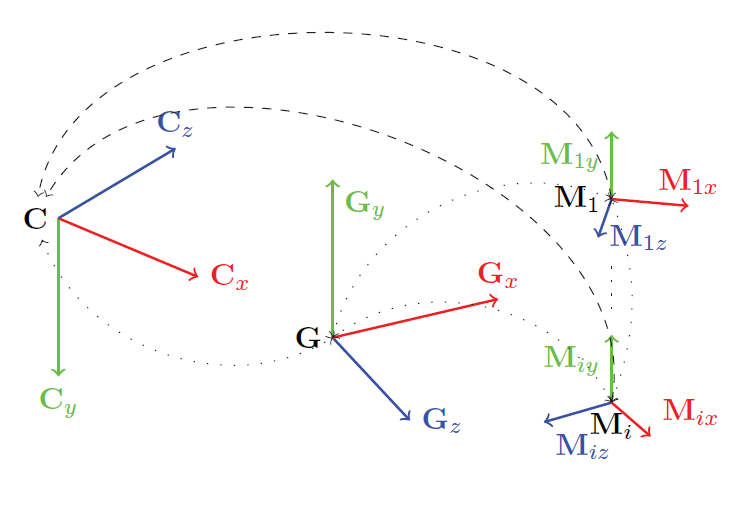
\includegraphics[width=0.9\textwidth]{img/coor.png}
                  	\caption{Coordinate Systems. Dashed connections are transformation matrices directly measured and dotted connections are transformation matrices to be optimized.}
							\end{minipage}
							\hspace{1em}
							\begin{minipage}{0.45\textwidth}
                    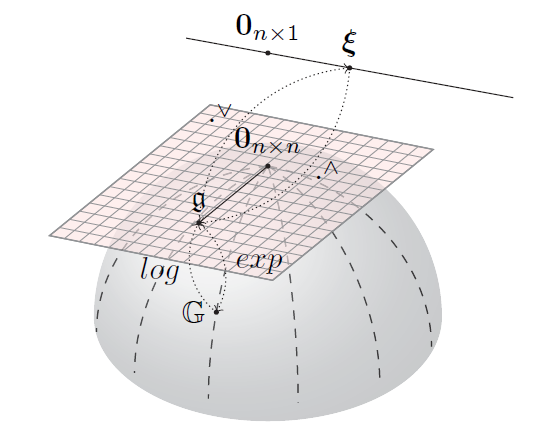
\includegraphics[width=0.9\textwidth]{img/lie.png}
								\caption{Mapping relationship among matrix Lie Group, Lie Algebra and the vector space.}
							\end{minipage}
						\end{figure}
\vspace{1em}
The pinhole camera model which is appropriate to most cameras is used in this work. We assume that the camera is supposed to be well-calibrated and the intrinsic parameters are precise since no optimization will be made on them.  

\end{myblock}


					\begin{myblock}{References}
						\footnotesize
						\bibliographystyle{abbrv}
						\bibliography{./bib}
					\end{myblock}\vfill

		}\end{minipage}\end{beamercolorbox}
	\end{column}
	\begin{column}{.57\textwidth}
		\begin{beamercolorbox}[center]{postercolumn}
			\begin{minipage}{.98\textwidth} % tweaks the width, makes a new \textwidth
				\parbox[t][\columnheight]{\textwidth}{ % must be some better way to set the the height, width and textwidth simultaneously
					\begin{myblock}{Methods}
\vspace{1em}
\begin{minipage}[0.3\textheight]{\textwidth}
\begin{columns}[T]
\begin{column}{0.5\textwidth}
\raggedright
\begin{enumerate}[label=,labelindent=\parindent,leftmargin=*]
\item This section details each step of the proposed method with a systematic chart shown in Fig.~\ref{fig:flowchart}.

\item[$\bullet$] ArUco detector implemented in OpenCV~\cite{aurcodetector} for fiducial detection and estimate pose with the RPnP algorithm~\cite{li2012robust}. The relative pose from $i^{th}$ marker to $j^{th}$ marker, if both viewed in $k^{th}$ camera frame, can be further computed as
\begin{equation}
{T_{\bold{M_i}}^{\bold{M}_j}}^{-1} = {T_{\bold{M}_j}^{\bold{M}_i}} = {T_{\bold{M}_i}^{\bold{C}_k}}^{-1}T_{\bold{M}_j}^{\bold{C}_k}
\end{equation}
By scanning all images collected, an initial pose graph $pg$ is incrementally established. A schematic diagram depicting the data structure of $pg$ is shown in Fig.~\ref{fig:dt_pg}.  

\item[$\bullet$] The aim of pose fusion is to refine the estimation of  ${{T}_{\bold{M}_i}^{\bold{M}_j}}$ by fusing all validated measurements obtained. After pose fusion process, a refined pose graph which better represents relative transformations of markers will be created. The Gauss-Newton method is used for pose fusion.

\item[$\bullet$] In order to establish optimal paths, the fused pose graph $pg_f$ is treated as an undirected graph with nodes, edges denoting markers and costs, respectively. Graph search method is used to find the origin which possess the minimum accumulated costs to all other vertices. The pose optimization is to further refine poses by minimizing per frame reprojection errors using the Levenberg–Marquardt (LM) algorithm~\cite{madsen1999methods}.
\end{enumerate}
\end{column}
\begin{column}{0.5\textwidth}
\begin{figure}
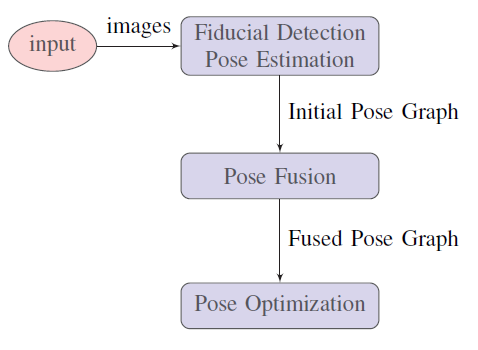
\includegraphics[width=0.72\textwidth]{img/flow.png}
\caption{Flowchart of proposed approach.}
\label{fig:flowchart}
\end{figure}
\begin{figure}
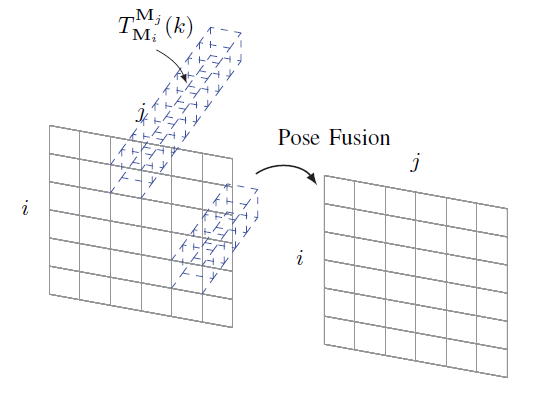
\includegraphics[width=0.72\textwidth]{img/ds.png}
\caption{Schematic diagram of the established initial pose graph $pg$ and pose graph $pg_{f}$ after pose fusion process.}
\label{fig:dt_pg}
\end{figure}
\begin{figure}
\centering
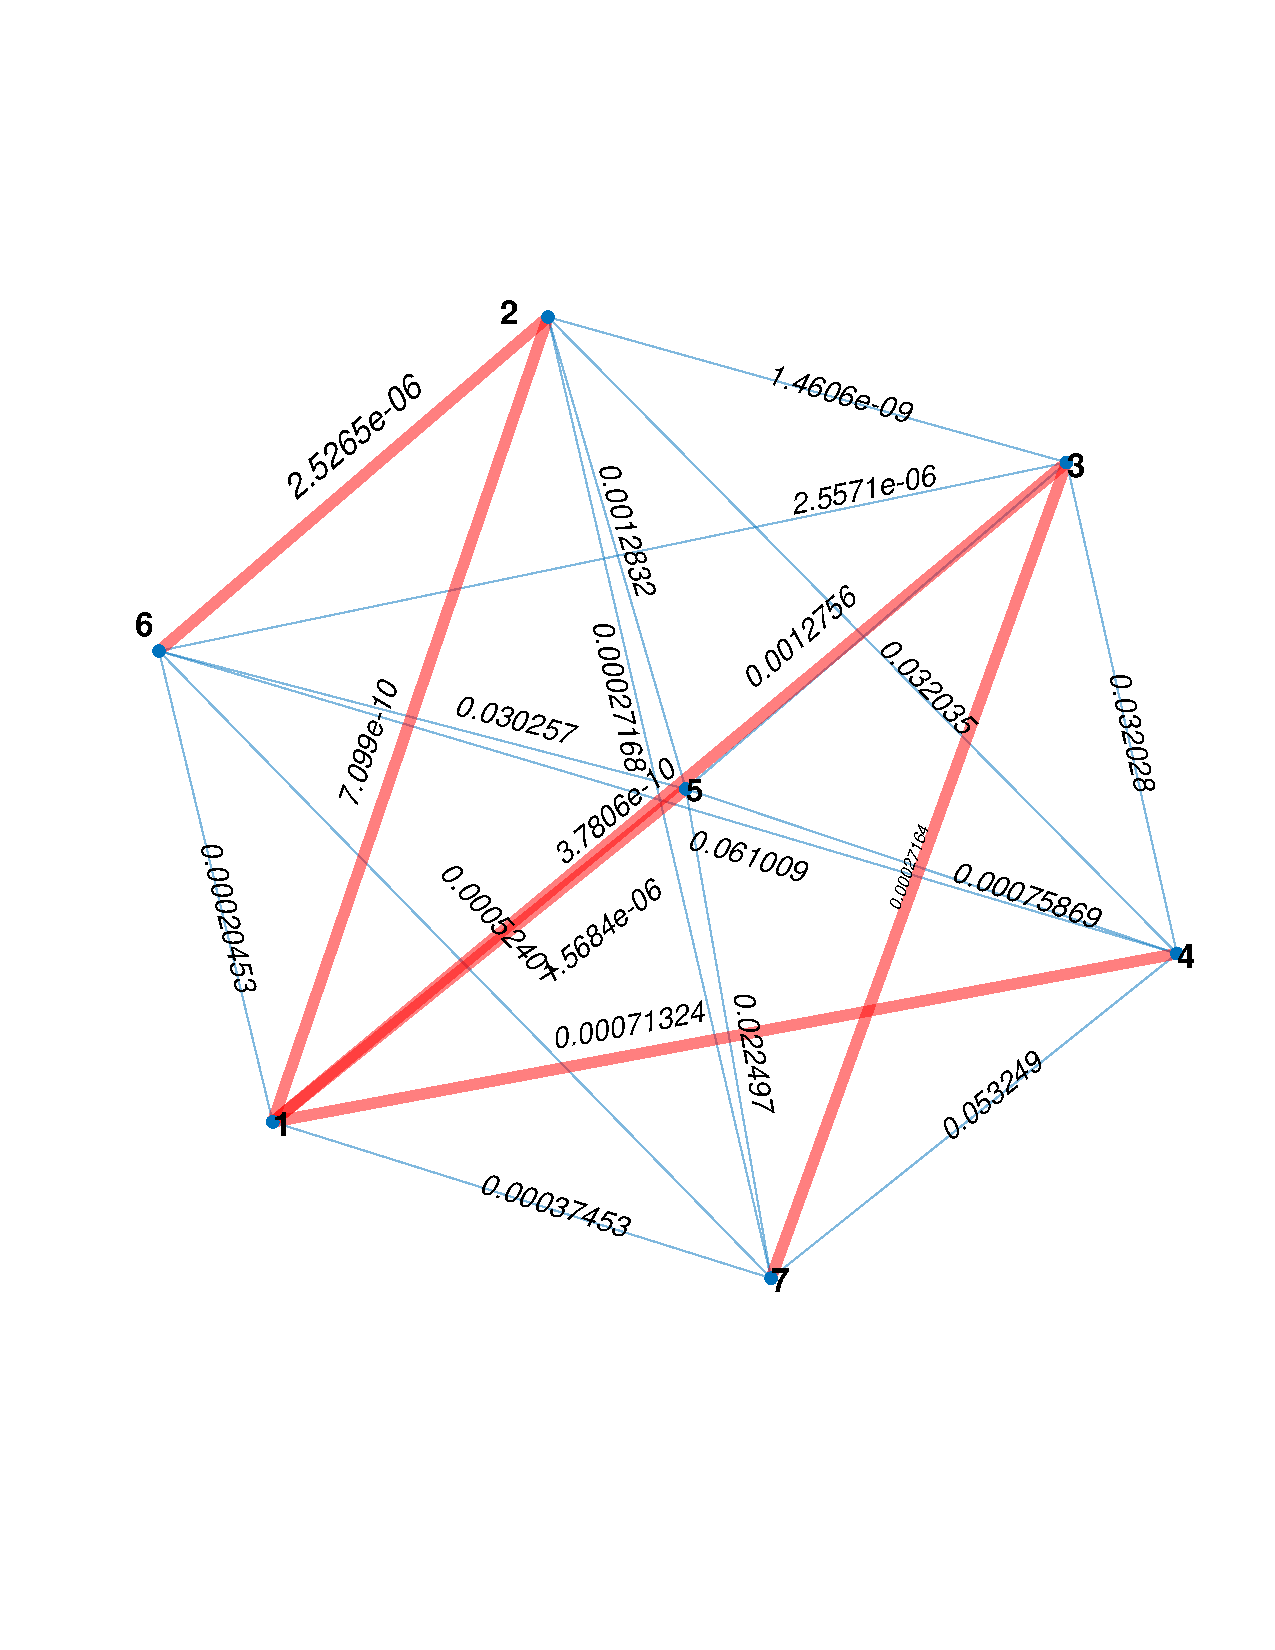
\includegraphics[scale=0.72]{img/graph}
\caption{Undirected Graph with blue dots denoting markers, solid light blue edges denoting costs. Red thick edges describe the minimum spanning tree obtained.}
\label{fig:ugraph}
\end{figure}
\end{column}
\end{columns}
\end{minipage}
\end{myblock}

\begin{myblock}{Results}
\begin{minipage}[0.3\textheight]{\textwidth}
\begin{columns}[T]
\begin{column}{0.33\textwidth}
\raggedright
\begin{enumerate}[label=,labelindent=\parindent,leftmargin=*]
\item[$\bullet$] Synthetic Mapping Test: 
\begin{figure}
\centering
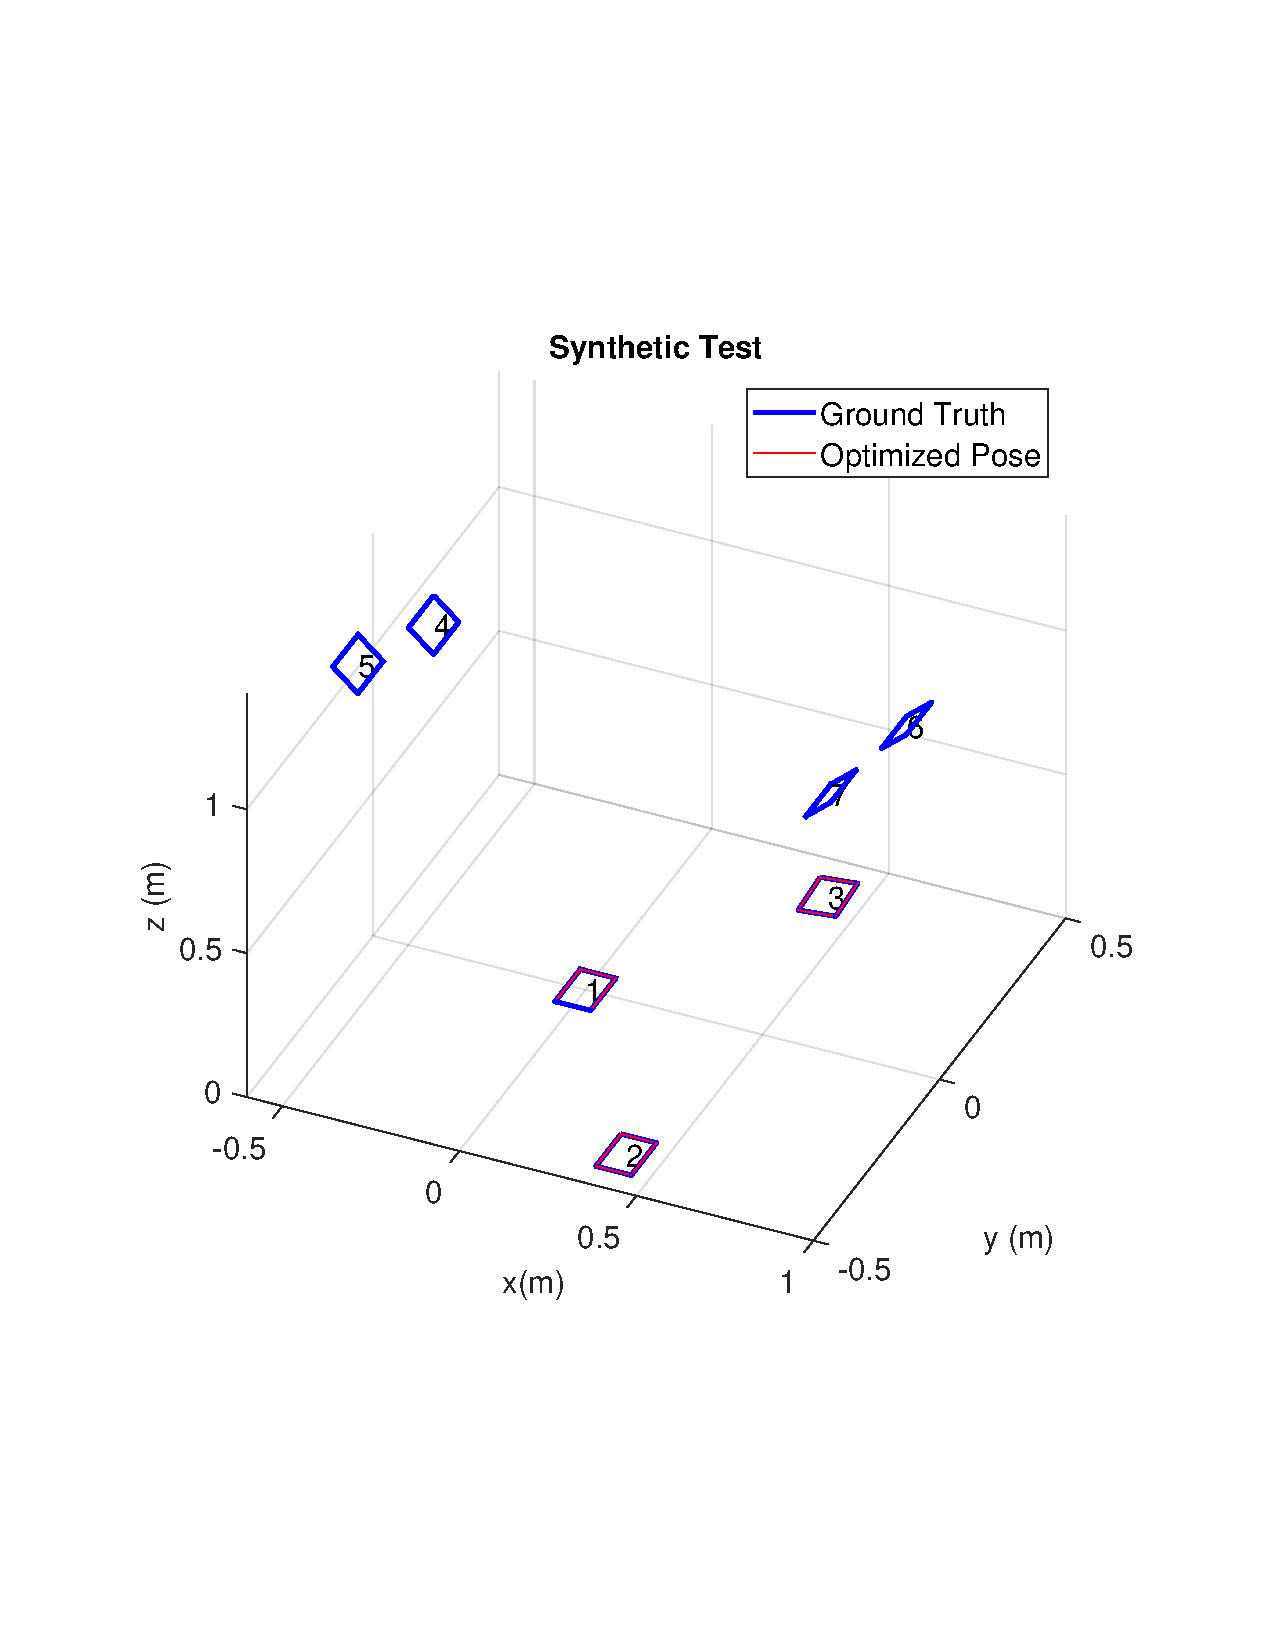
\includegraphics[width=1.0\textwidth]{img/synthetic_3d_new}
\caption{Synthetic Mapping result. Blue squares denote ground truth and red squares denote the optimized markers' pose.}
\label{fig:synthetic_3d}
\end{figure}
\begin{figure}
\centering
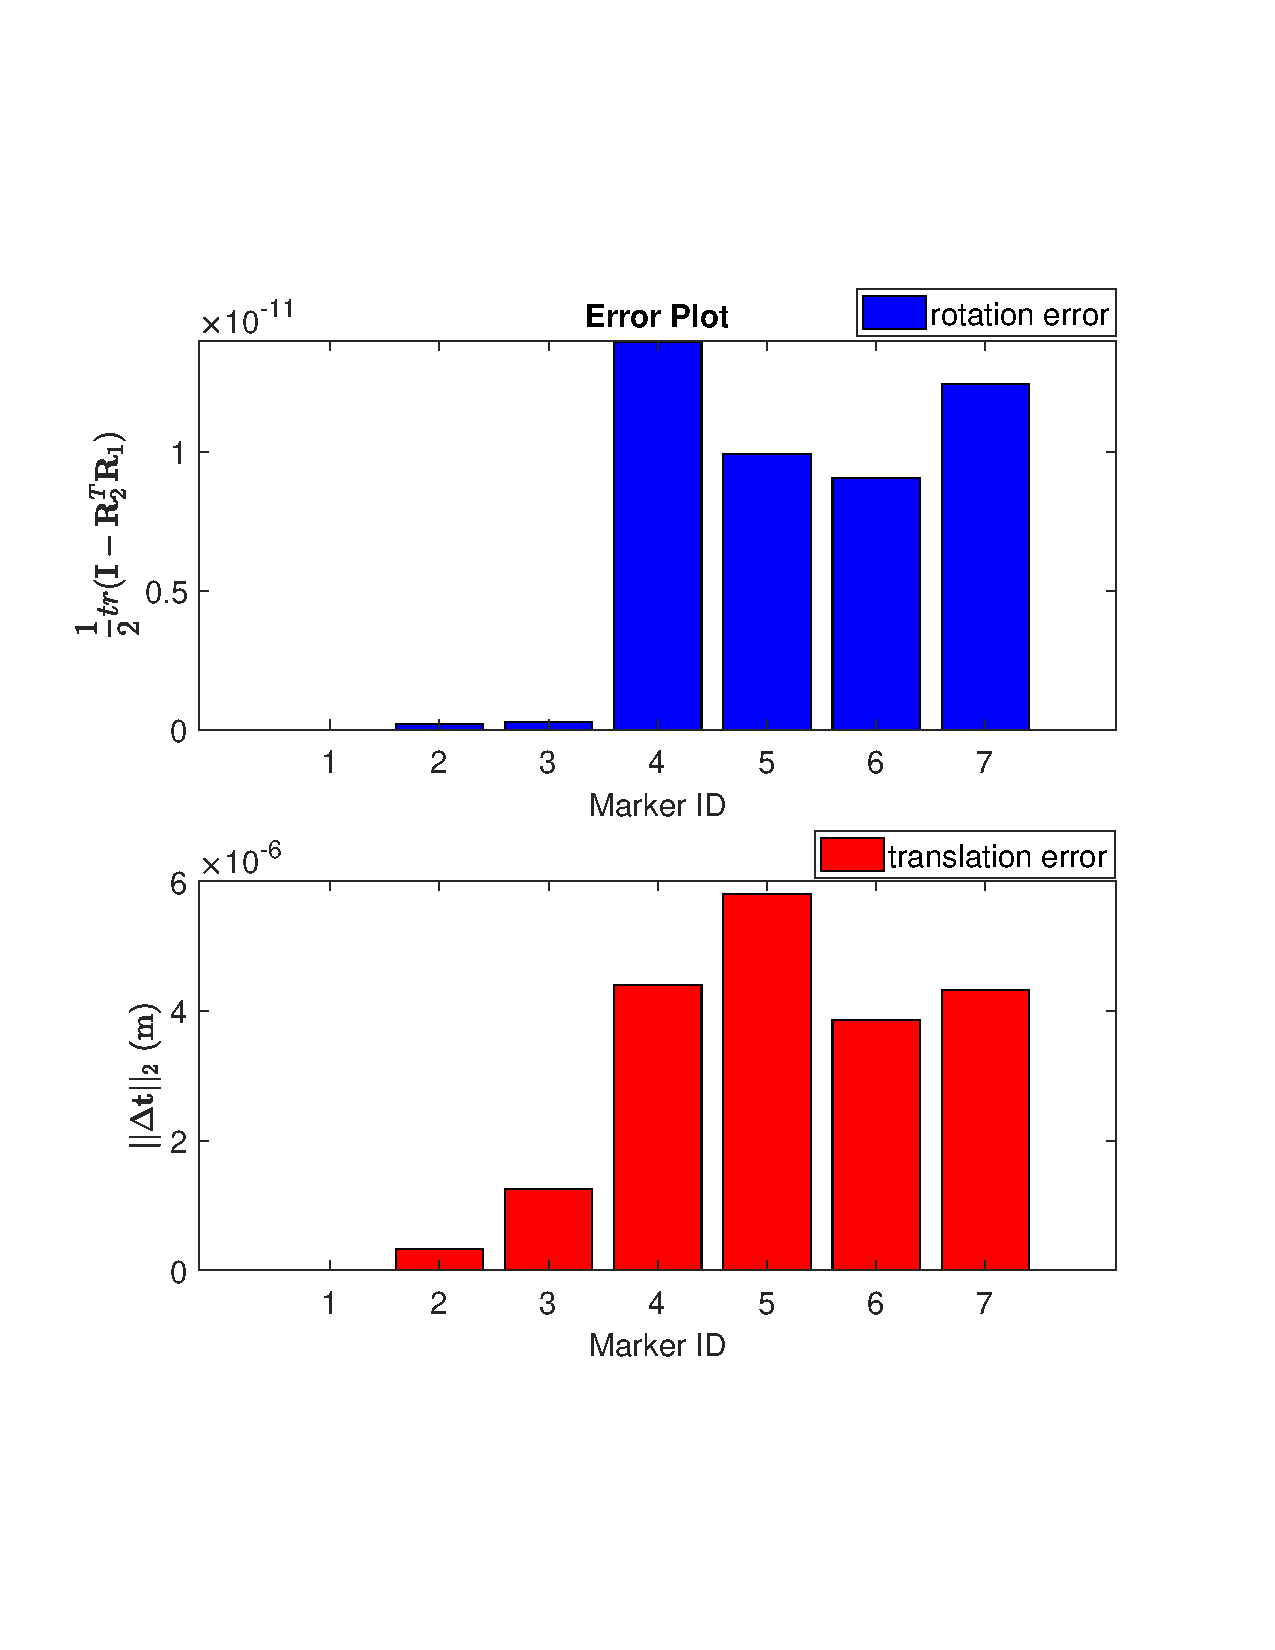
\includegraphics[width=1.0\textwidth]{img/synthetic_rt_new}
\caption{Rotation and translation error analysis. Marker $1$ is set as the origin. Consequently, its rotation and translation errors are zero. Translation errors are measured in meters.}
\label{fig:synthetic_rt}
\end{figure}
\end{enumerate}
\end{column}

\begin{column}{0.33\textwidth}
\begin{enumerate}[label=,labelindent=\parindent,leftmargin=*]
\item[$\bullet$] Box Test: 
\begin{figure}
\centering
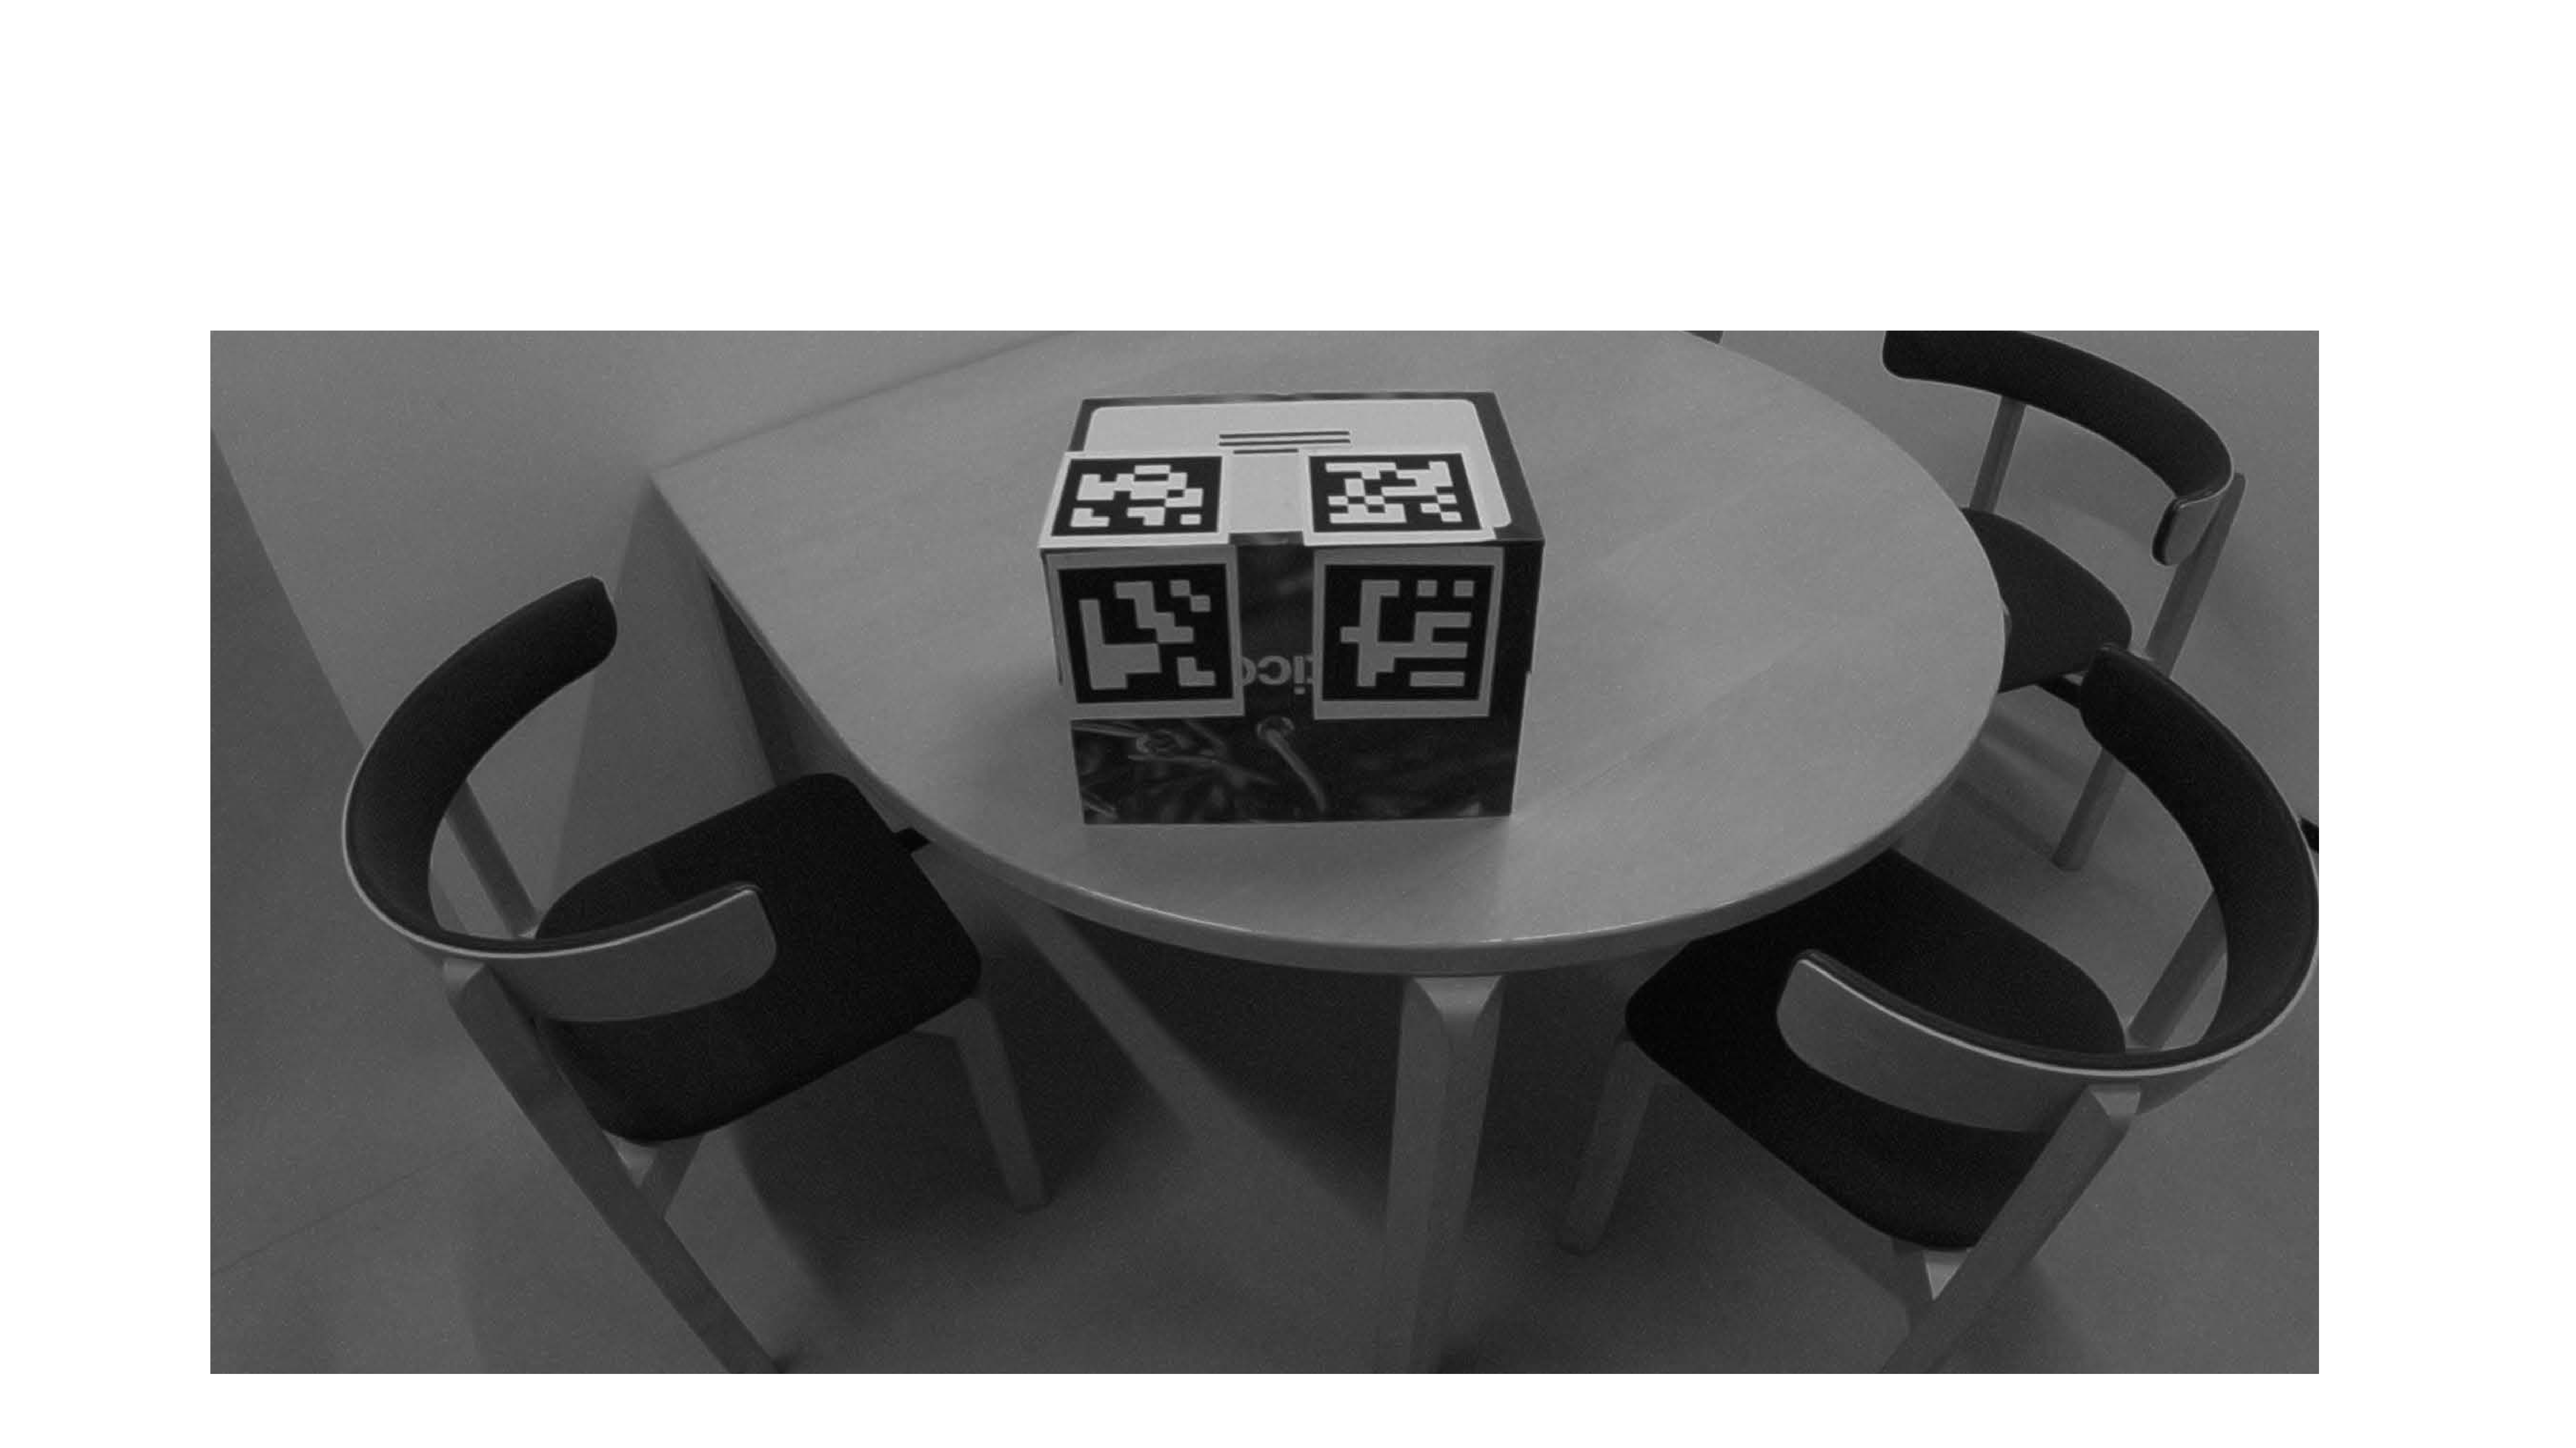
\includegraphics[width=0.6\textwidth]{img/box_snap}
\caption{Experiment setup: left is the snapshot of "box" experiment.}
\label{fig:snap_table_box}
\end{figure}
\begin{figure}
\centering
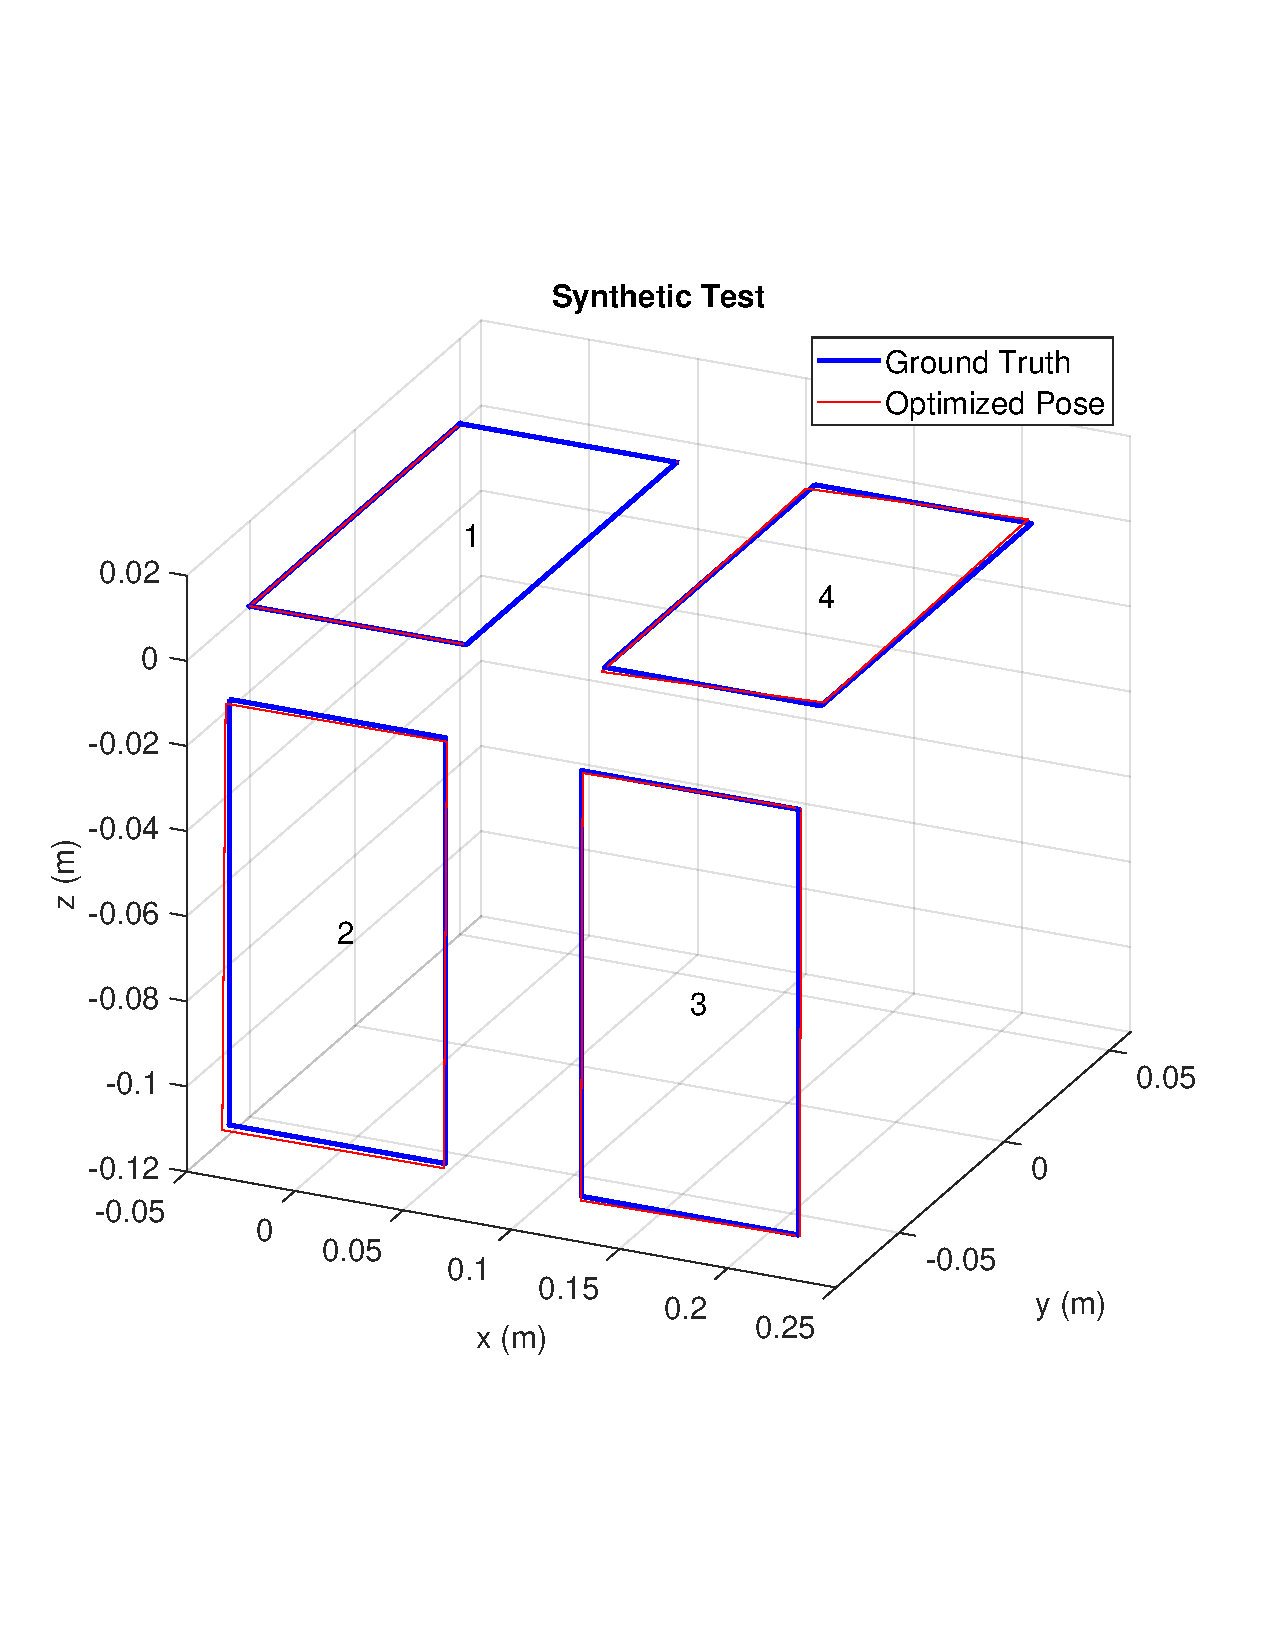
\includegraphics[width=1.0\textwidth]{img/box_3d_new}
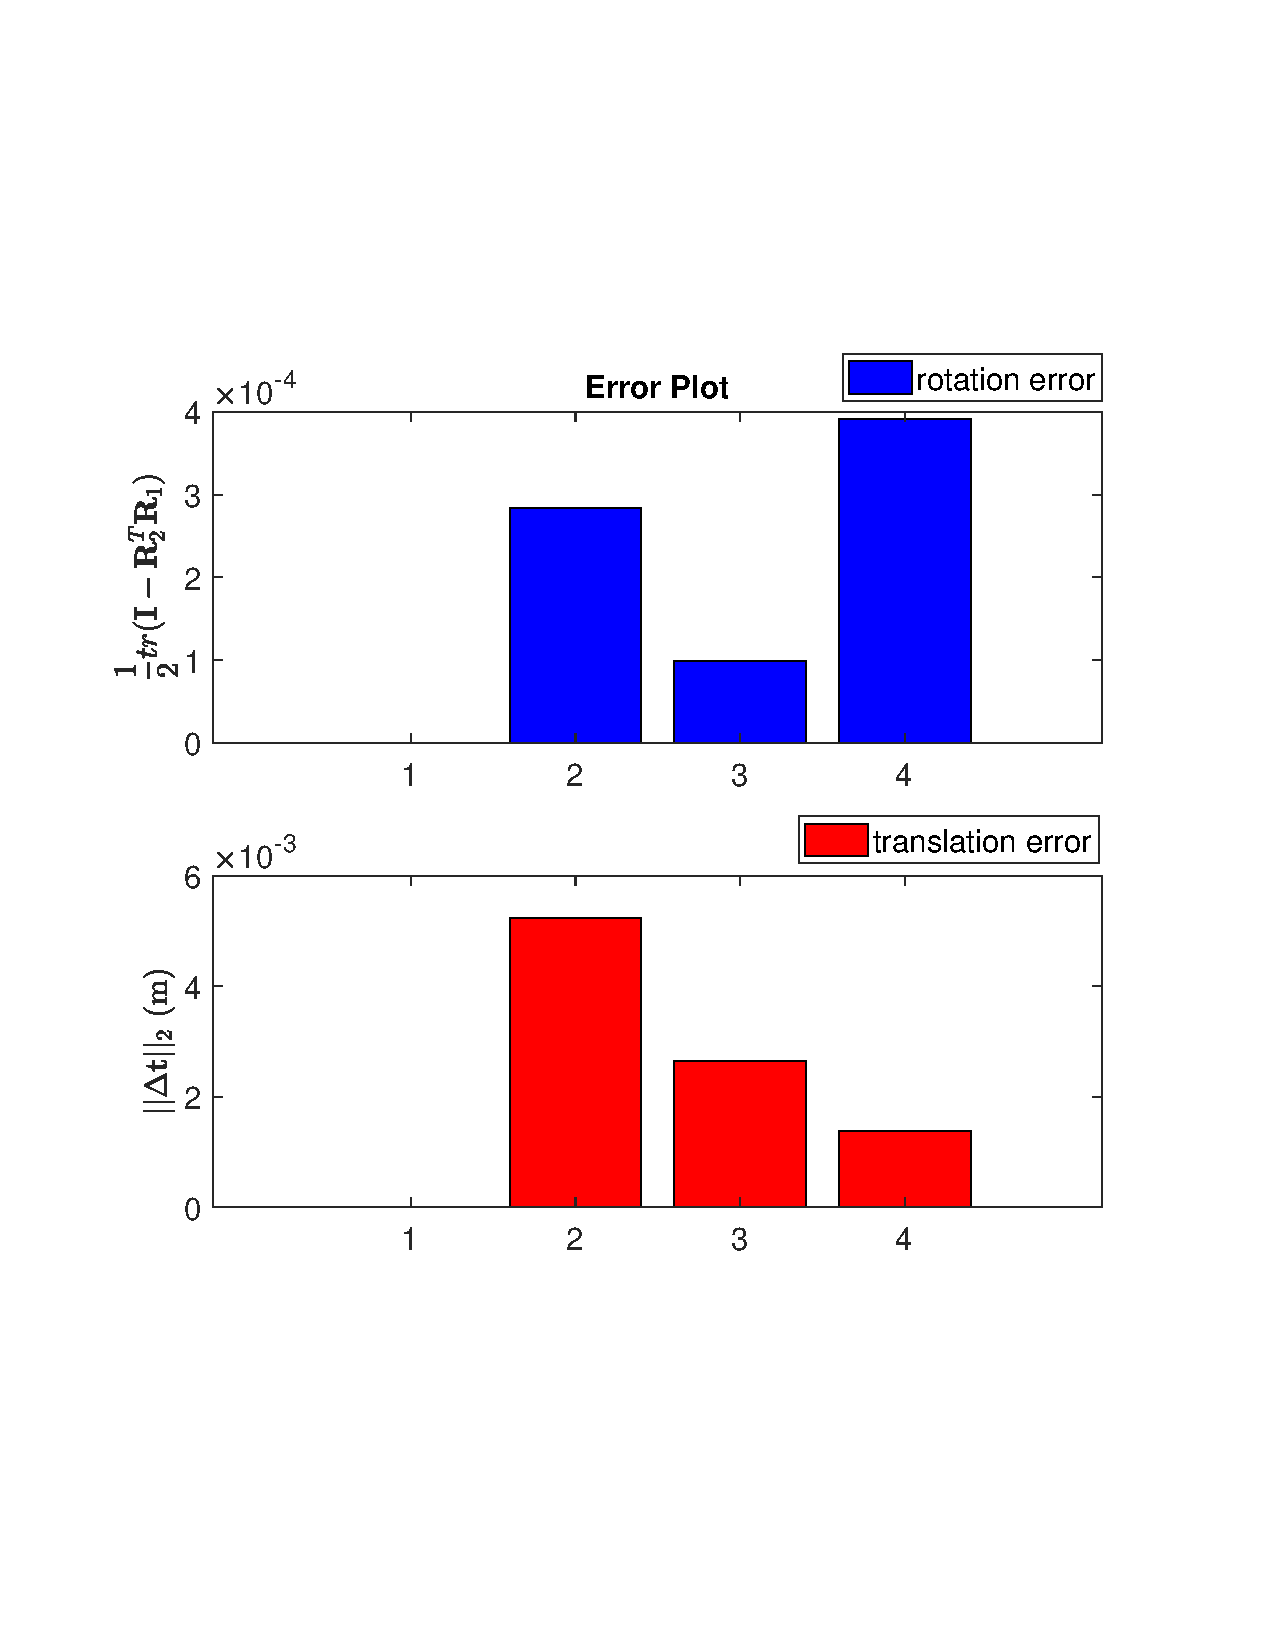
\includegraphics[width=1.0\textwidth]{img/box_rt_new}
\caption{Mapping result and error plots from "box" experiment. Marker $1$ is the origin so its erros are zero.}
\label{fig:box_res}
\end{figure}
\end{enumerate}
\end{column}

\begin{column}{0.33\textwidth}
\begin{enumerate}[label=,labelindent=\parindent,leftmargin=*]
\item[$\bullet$] Pose Estimation Test: the GoPro Hero 6 is used
to capture images with a resolution of 2.7K (2704 × 1520).
\begin{figure}
\centering
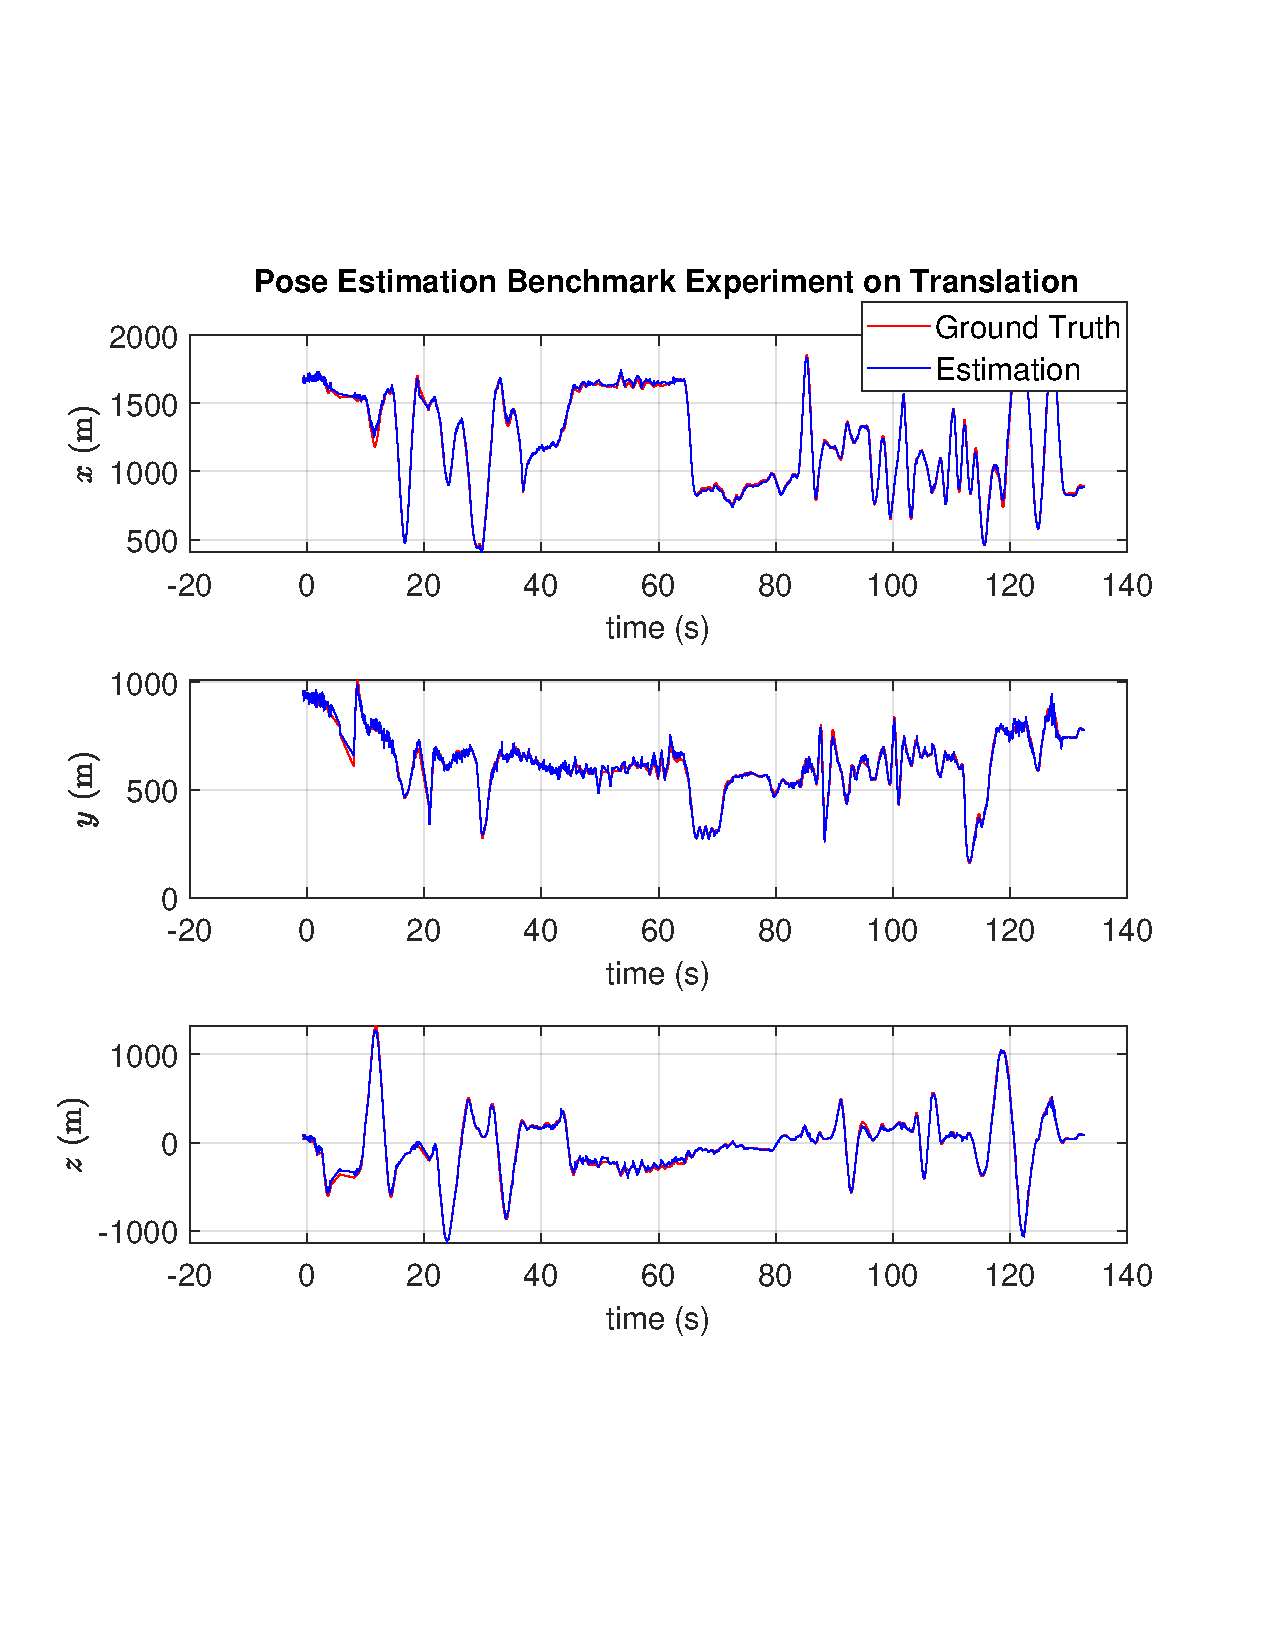
\includegraphics[width=1.0\textwidth]{img/xyz_new}
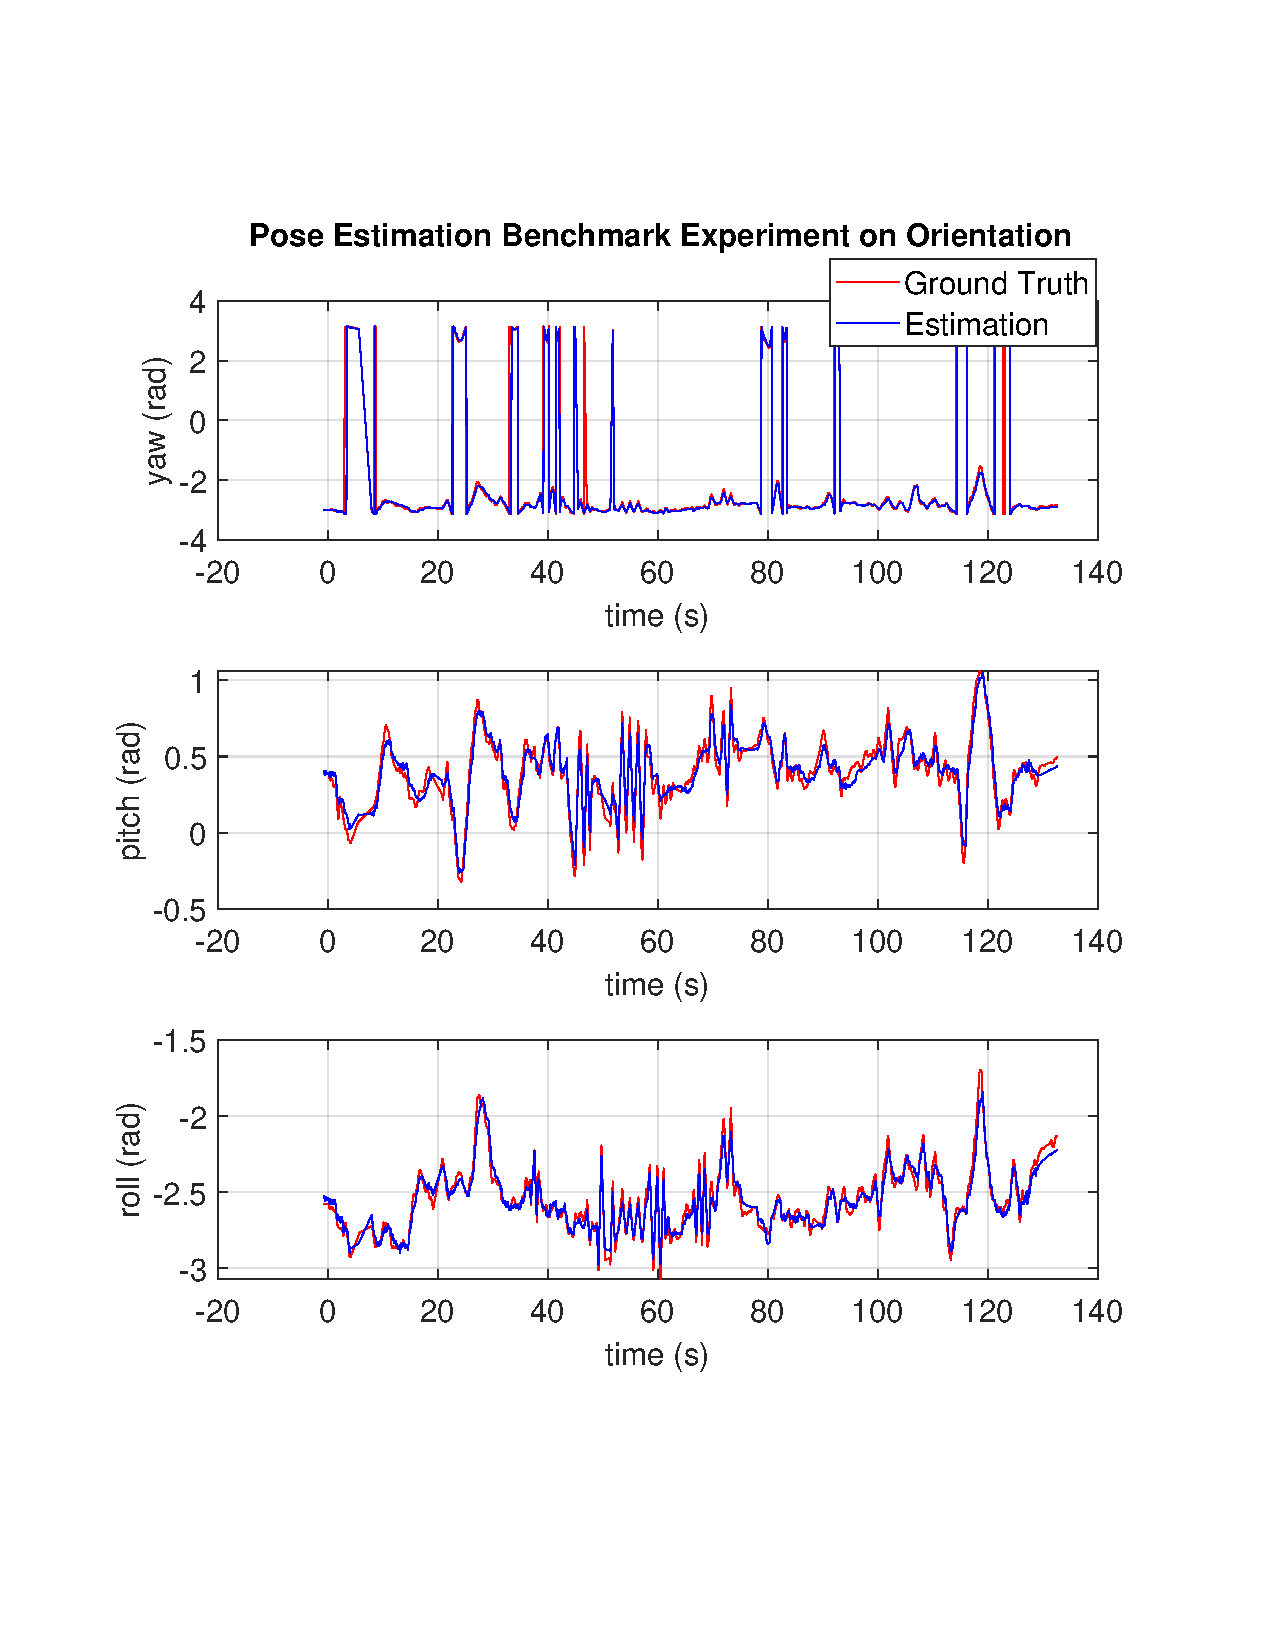
\includegraphics[width=1.0\textwidth]{img/rpy_new}
\caption{Benchmark Test of pose estimation from fiducial map (blue) and ground truth (red).}
\label{fig:benchmark}
%\includegraphics[width=4cm,height=4cm]{window}
%\includegraphics[width=4cm,height=4cm]{ls_table}
%\caption{Snapshots of markers.}
\end{figure}
\end{enumerate}
\end{column}

\end{columns}
\end{minipage}
\end{myblock}\vfill
\begin{myblock}{Acknowledgement}
This work is supported by the Innovation Fund Denmark via project UAV-QMS.
\end{myblock}\vfill

		}\end{minipage}\end{beamercolorbox}
	\end{column}
\end{columns}
\end{frame}
\end{document}
